% ==============================================================================
% sci_s5_sim_analysis.tex — SCI/SICE tutorial Session 5: simulator & analysis
% tools, advanced topics, Q&A (15:30-16:30)
% SCI/SICE チュートリアル セッション5: シミュレータ・解析ツールの活用と
% 発展的テーマの紹介と質疑（15:30-16:30）
% ==============================================================================

% Fallback so this chapter still builds standalone (make chapter NAME=sci_s5_sim_analysis)
% before chapters/sci_intro.tex has run. In the full deck sci_intro defines the
% real \scisessionmap first, so this no-ops there.
\providecommand{\scisessionmap}[1]{}

% ------------------------------------------------------------------
\begin{frame}{地図: 今ここ}
  \begin{columns}[T]
    \begin{column}{0.5\textwidth}
      \centering
      \resizebox{\columnwidth}{!}{\scisessionmap{5}}
    \end{column}
    \begin{column}{0.47\textwidth}
      \small
      S4 で飛ばした結果を，本セッションではシミュレータと解析ツールで
      裏付ける。「実験」の次にくる「解析」と「教育」のフェーズにあたる。

      \vspace{0.5em}

      \begin{block}{本日の最後に扱うもの}
        \footnotesize
        3層シミュレーション $\to$ SILS 実習 $\to$ 解析ツールと教育教材 $\to$
        研究・発展テーマ $\to$ 質疑
      \end{block}
    \end{column}
  \end{columns}
\end{frame}

% ------------------------------------------------------------------
\begin{frame}{要点3つ}
  \begin{enumerate}
    \item StampFly のシミュレーションは目的の異なる3層で構成され，
          層3（SILS）は実ファームを無改変で走らせる
    \item 学習者が実装した推定器・制御器は，L1 Topic API 経由で
          既存の実装と差し替えられる
    \item 実習 5/8 で書いた PID コードは，実機を飛ばす前に SILS で
          検証してから持ち帰れる（本セッション後半で実習）
  \end{enumerate}

  \vspace{0.5em}

  \begin{alertblock}{本セッションの立ち位置}
    \small
    S4 までは1機の StampFly を飛ばす話だった。ここからは，飛ばさずに
    検証する方法と，1機から先の広がりを扱う
  \end{alertblock}
\end{frame}

% ------------------------------------------------------------------
\begin{frame}{シミュレーションの3層構造}
  \begin{center}
    \resizebox{0.95\textwidth}{!}{% sci_sim_layers.tex — Three simulation layers for the SCI tutorial (S5)
% シミュレーションの3層構造図。SCIチュートリアル S5 用。
%
% Source: docs/architecture/simulation-policy.md §2 (three-layer table),
% §2 "層の関係" (layer 2 is independently positioned, NOT a simplified
% version of layer 3), and §4 (model-match gate).
% 出典: docs/architecture/simulation-policy.md §2（3層構造の表）、
% §2「層の関係」（層2は層3の簡略版ではなく独立した位置づけ）、
% §4（モデル一致ゲート）。
%
% Author's 2nd-round review (2026-09): the previous version drew a FLOW
% (three boxes side by side, left-to-right arrow chain) — the reviewer's
% point was that this reads as a pipeline/flowchart, not as layers. This
% version redraws the three tiers as STACKED HORIZONTAL BANDS (layer1 on
% top, matching the top-to-bottom row order used by the "対応表"/"table"
% frame elsewhere in this chapter), each band self-contained (title / what
% it provides / tool / what it verifies). Short vertical arrows between
% adjacent bands carry the teaching narrative from S5 item 1:
%   モデルがある(層1) -> 実ログで検証できる(層2) -> 飛ばす前にSILSで検証できる(層3)
% The model-match gate is drawn as a SIDE box (not another stacked band,
% since it is not itself a simulation tier — it is the §4 procedure that
% cross-checks layer3's identified plant against layer1's real-machine
% reference), connected by right-angle arrows to layer1 and layer3 only.
%
% 著者の第2ラウンドレビュー（2026-09）: 旧版は3つの箱を横に並べ矢印で
% つなぐ「フロー」だった — 指摘は「層ではなくフローに見える」というもの。
% 本版は3層を縦積みの横長バンドとして描き直す（層1を上に、本章の
% 「対応表」フレームの行順=層1→層2→層3の上から下という並びと揃える）。
% 各バンドは自己完結（タイトル/提供するもの/ツール/何を検証するか）。
% 隣接バンド間の短い垂直矢印が、S5 item 1 の説明の流れを運ぶ:
%   モデルがある(層1) -> 実ログで検証できる(層2) -> 飛ばす前にSILSで検証できる(層3)
% モデル一致ゲートは「層」ではない（§4の判定手順であり、層3で同定した
% プラントを層1の実機基準値と突き合わせる）ため、積み重ねた4つ目のバンドに
% はせず、層1・層3の2つだけに直角矢印で接続するサイド箱として描く。
\documentclass[border=10pt]{standalone}
\usepackage{tikz}
\usetikzlibrary{arrows.meta, positioning, calc}
\usepackage{luatexja}
\usepackage[match]{luatexja-fontspec}
% Cross-platform font: Hiragino (macOS) → Yu Gothic (Windows) → Noto (Linux)
% クロスプラットフォーム: ヒラギノ (macOS) → 游ゴシック (Windows) → Noto (Linux)
\usepackage{ifthen}
\newboolean{jfontset}\setboolean{jfontset}{false}
\IfFontExistsTF{Hiragino Kaku Gothic ProN}{%
  \setmainjfont{Hiragino Kaku Gothic ProN}%
  \setsansjfont{Hiragino Kaku Gothic ProN}%
  \setboolean{jfontset}{true}}{}
\ifthenelse{\boolean{jfontset}}{}{%
  \IfFontExistsTF{Yu Gothic}{%
    \setmainjfont{Yu Gothic}%
    \setsansjfont{Yu Gothic}%
    \setboolean{jfontset}{true}}{}}
\ifthenelse{\boolean{jfontset}}{}{%
  \IfFontExistsTF{Noto Sans CJK JP}{%
    \setmainjfont{Noto Sans CJK JP}%
    \setsansjfont{Noto Sans CJK JP}}{}}

\begin{document}

\definecolor{s1color}{RGB}{0, 100, 180}
\definecolor{s2color}{RGB}{40, 140, 60}
\definecolor{s3color}{RGB}{150, 90, 20}
\definecolor{gatecolor}{RGB}{170, 30, 30}
\definecolor{gray1}{RGB}{120, 120, 120}

% Plain-LaTeX helper macros for the colored text lines inside each band
% 帯の中の色付きテキスト用マクロ
\newcommand{\ttier}[2]{{\bfseries\normalsize\color{#1}#2}}
\newcommand{\tsub}[1]{{\scriptsize\color{black!55}#1}}

\begin{tikzpicture}[
    band/.style={
      rectangle, rounded corners=4pt, draw=#1, line width=1.5pt,
      fill=#1!8, minimum width=108mm, minimum height=13mm,
      align=left, inner xsep=4mm, inner ysep=0.8mm
    },
    gatebox/.style={
      rectangle, rounded corners=4pt, draw=gatecolor, line width=1.3pt,
      fill=gatecolor!7, minimum width=50mm, minimum height=28mm,
      align=left, inner xsep=3mm, inner ysep=2mm
    },
    relarr/.style={-{Stealth[length=3mm]}, line width=1.5pt, gray1},
    garr/.style={-{Stealth[length=3mm]}, line width=1.4pt, gatecolor},
  ]

  % Three STACKED bands, top (Layer 1, design-time) to bottom (Layer 3,
  % SILS) — matches the row order of the "対応表" table elsewhere in this
  % chapter (層1/層2/層3 top-to-bottom). This is the core fix for the
  % reviewer's "flow, not layers" complaint: full-width horizontal bars
  % stacked vertically, not boxes chained left-to-right.
  %
  % Line budget: each band is title + 2 SHORT sublines (not long sentences)
  % so every line fits in ONE row at this width without wrapping — a
  % wrapped line silently doubles a band's height and was the actual cause
  % of an earlier revision's 91pt (32mm) frame overflow (verified by
  % rebuilding and reading the log, not guessed).
  % 3つの帯を縦に積む。上（層1・設計時）から下（層3・SILS）へ — 本章の
  % 「対応表」の行順（層1/層2/層3、上から下）と揃える。「フローであって
  % 層ではない」という指摘への核心的な修正: 横長のバーを縦に積むのであって、
  % 箱を左から右へ連鎖させるのではない。
  %
  % 行数の設計: 各帯はタイトル＋短い2行（長い一文にしない）とし、この幅で
  % 折り返さず1行に収める — 行の折り返しは帯の高さを暗黙に倍増させ、
  % 以前の版でフレームが91pt（32mm）溢れた実際の原因だった（推測ではなく
  % 再ビルドしてログを読んで確認済み）。
  \node[band=s1color] (S1) at (0, 0) {%
    \begin{minipage}{99mm}\raggedright
      \ttier{s1color}{層1: 設計用線形モデル}\\[1.5pt]
      \tsub{$G(s){=}b\,e^{-Ls}/(s(Ts{+}1))$（伝達関数として扱う）}\\[1pt]
      \tsub{\texttt{sf sysid rate-fit} で同定 $\to$ 設計・ループ整形の正}
    \end{minipage}%
  };
  \node[band=s2color, below=5mm of S1] (S2) {%
    \begin{minipage}{99mm}\raggedright
      \ttier{s2color}{層2: 実ログ駆動オフライン再生}\\[1.5pt]
      \tsub{層1と同じ$G(s)$＋飽和等，制御則はPython移植}\\[1pt]
      \tsub{実ログ外乱で駆動（\texttt{analysis/scripts/}）$\to$ A/B判定の正}
    \end{minipage}%
  };
  \node[band=s3color, below=5mm of S2] (S3) {%
    \begin{minipage}{99mm}\raggedright
      \ttier{s3color}{層3: SILS（実ファーム + MuJoCo）}\\[1.5pt]
      \tsub{非線形6自由度のプラント＋実ファームC++そのもの}\\[1pt]
      \tsub{Code/Param Identity $\to$ 飛ばす前のシステム全体検証}
    \end{minipage}%
  };

  % Short vertical arrows between adjacent bands, straight (no bend needed
  % since the bands already share the same x-center), centered on the gap
  % between bands. Each carries one clause of the S5 item-1 narrative.
  % 隣接する帯の間の短い垂直矢印。帯は既に同じx中心を共有しているため
  % 折れ曲がり不要の直線。帯間のギャップの中央に配置し、各矢印がS5 item 1
  % の説明文の一節を運ぶ。
  \draw[relarr] (S1.south) -- (S2.north);
  \draw[relarr] (S2.south) -- (S3.north);

  % Labels sit to the RIGHT of each vertical arrow (not on top of the
  % line — T2), inside the inter-band gap so they cannot collide with any
  % band's text (the gap is empty space between two boxes) or with the
  % gate/bus on the right margin (labels stop well before that region).
  % ラベルは各垂直矢印の右側に置く（線の上に乗せない — T2）。帯間ギャップ
  % （2つの箱の間の空白）の中に収まるため、帯のテキストとも右マージンの
  % ゲート/バスとも衝突しない（ラベルはその領域よりずっと手前で止まる）。
  \node[font=\scriptsize, text=gray1, anchor=west]
    at ($(S1.south)!0.5!(S2.north)+(4mm,0)$) {実ログで照合};
  \node[font=\scriptsize, text=gray1, anchor=west]
    at ($(S2.south)!0.5!(S3.north)+(4mm,0)$) {飛行前検証};

  % Model-match gate (§4): a SIDE box, not a fourth stacked layer — it is
  % the verification procedure that cross-checks layer3's identified
  % plant against layer1's real-machine reference, so it connects to
  % layer1 AND layer3 only (never layer2, which the policy explicitly
  % keeps independent of layer3 — §2 "層の関係"). Vertically centered on
  % the S1-S3 span (== S2's height, since bands are symmetric).
  % モデル一致ゲート（§4）: 「層」ではなくサイド箱 — 層3で同定したプラント
  % を層1の実機基準値と突き合わせる判定手順そのものなので、層1・層3にのみ
  % 接続する（層2には繋がない。方針書§2「層の関係」で層2は層3と独立と
  % 明記されているため）。S1〜S3の全体スパンの中央（帯が対称なのでS2の高さ
  % と同じ）に配置。
  \node[gatebox, right=20mm of S2] (GATE) {%
    \begin{minipage}{43mm}\raggedright
      \ttier{gatecolor}{モデル一致の合否判定}\\[3pt]
      \tsub{層3ログを層1と同一手順で同定}\\[2pt]
      \tsub{$(b,L,T)$ を層1基準値と比較}\\[2pt]
      \tsub{（\texttt{sf sils sysid-gate}）}
    \end{minipage}%
  };

  % Right-angle routing from Layer 1 / Layer 3 into the gate. The corner
  % x-coordinate is taken from GATE (via "-|", which reads x from its
  % RIGHT operand) so the vertical run lands exactly on GATE's north/south
  % edge midpoint — an edge, not a corner (T4f) — with a >=8mm straight
  % trunk before each arrowhead.
  % 層1／層3からゲートへの直角配線。コーナーのx座標はGATE側から取る
  % （"-|" は右側の被演算子からxを読む）ため、垂直区間はGATEのnorth/south
  % 辺の中点に正確に着地する（角ではなく辺 — T4f）。矢頭前に8mm以上の
  % 直線区間を確保する。
  \draw[garr] (S1.east) -- (S1.east -| GATE) -- (GATE.north);
  \draw[garr] (S3.east) -- (S3.east -| GATE) -- (GATE.south);

  % Labels for the gate's two inputs, placed above/below their horizontal
  % run (clear of the S1/S3 bands to the left and the GATE box to the
  % right — this horizontal segment is empty space by construction).
  % ゲートへの2入力のラベル。それぞれの水平区間の上/下に配置する
  % （左のS1/S3帯とも右のGATE箱とも構造上ぶつからない空白領域）。
  \node[font=\scriptsize, text=gatecolor, anchor=south]
    at ($(S1.east)!0.5!(S1.east -| GATE)+(0,1mm)$) {実機同定値（基準）};
  \node[font=\scriptsize, text=gatecolor, anchor=north]
    at ($(S3.east)!0.5!(S3.east -| GATE)+(0,-1mm)$) {同一パイプラインで同定};

\end{tikzpicture}
\end{document}
}
  \end{center}

  {\footnotesize 目的の異なる3層を使い分ける。詳細は \code{docs/architecture/simulation-policy.md} を参照}
\end{frame}

% ------------------------------------------------------------------
\begin{frame}{層1・層2: 設計モデルとログ再生}
  \begin{exampleblock}{層1: 設計用線形モデル}\small
    $G(s) = b\,e^{-Ls}/(s(Ts+1))$ を \code{sf sysid rate-fit} で実飛行ログから
    同定し，制御設計とループ整形の基準とする（S4 で扱った同定と同じ枠組み）
  \end{exampleblock}

  \vspace{0.5em}

  \begin{block}{層2: 実ログ駆動オフライン再生}\small
    層1のモデルと Python に移植した制御則を，実機ログから再構成した
    実外乱・実指令で駆動する閉ループ再生。パラメータ変更の A/B 判定の基準
  \end{block}

  {\footnotesize \code{analysis/scripts/} 配下の Python 群。ヨー$\kappa$修正のリプレイ一致
  0.0〜0.7\%，ALT\_HOLD 再生誤差約8\%という精度で検証できている}
\end{frame}

% ------------------------------------------------------------------
\begin{frame}{層3: SILS}
  \begin{block}{Code Identity と Parameter Identity}\small
    SILS（Software-in-the-Loop Simulation: 実ファームをホスト PC 上で
    物理シミュレーションと閉ループ実行する検証手法）は，
    MuJoCo（非線形6自由度の物理エンジン）と\textbf{実ファーム C++ そのもの}を，
    実機と同じソース・同じパラメータで走らせる
  \end{block}

  \vspace{0.5em}

  \begin{itemize}\small
    \item 状態機械・推定器・フェイルセーフを含むシステム全体の検証ベンチ
    \item 推定器を ESKF から相補フィルタに差し替えても，ベンチは無改変で
          同じ検証ができる（アルゴリズムの中身に依存しない設計）
    \item シナリオファイル（\code{.scn}）と合格基準（\code{.expect}）の組で自動判定する。
          \code{sf sils regression} でまとめて実行できる
  \end{itemize}
\end{frame}

% ------------------------------------------------------------------
\begin{frame}{モデル一致の合否判定}
  \begin{block}{Code Identity を使った検証}\small
    実機ログに使うのと同じ同定パイプラインを，SILS が生成したログにも
    そのまま適用し，$(b, L, T)$ を実機同定値と比較する（\code{sf sils sysid-gate}）
  \end{block}

  \vspace{0.5em}

  \begin{table}
    \centering\small
    \begin{tabular}{lc}
      \hline
      \textbf{指標} & \textbf{許容差（判定条件）} \\
      \hline
      ステップ応答立ち上がり時定数 & $\pm20\%$ \\
      gyro RMS & $\pm50\%$ \\
      \hline
    \end{tabular}
  \end{table}

  {\footnotesize Yaw は反トルク零点を持ち，現行の3パラメータフィットでは表現しきれない。
  軸ごとの物理特性に応じて，公称モデル1点比較と摂動族での検証を使い分ける}
\end{frame}

% ------------------------------------------------------------------
\begin{frame}[fragile]{VPython と Genesis}
  \begin{table}
    \centering\small
    \begin{tabular}{lll}
      \hline
      & \textbf{特徴} & \textbf{用途} \\
      \hline
      VPython & 軽量，ブラウザ3D表示，センサモデル充実 & 制御学習，SILS/HILS\footnotemark \\
      Genesis & 高精度物理エンジン，2000\,Hz 物理演算 & 高精度シミュレーション \\
      \hline
    \end{tabular}
  \end{table}
  \footnotetext{\scriptsize HILS（Hardware-in-the-Loop Simulation）:
  実機を接続した検証。本エコシステムではファーム側未対応}

  \vspace{0.5em}

  \begin{sflisting}[basicstyle=\ttfamily\scriptsize]{コマンド}
sf sim run vpython
sf sim run genesis
  \end{sflisting}

  {\footnotesize AtomS3 + Atom JoyStick を USB HID モードで使い，実機と同じ操縦感で
  シミュレータを飛ばせる}
\end{frame}

% ------------------------------------------------------------------
\begin{frame}[fragile]{sf sils コマンド一覧}
  \begin{table}
    \centering\footnotesize
    \begin{tabular}{ll}
      \hline
      \textbf{サブコマンド} & \textbf{機能} \\
      \hline
      \code{build}      & SILS ホストベンチをビルド \\
      \code{run}         & 閉ループを実行しバンドルを書き出す \\
      \code{scenario}    & \code{.scn} シナリオを実行し合否判定 \\
      \code{regression}  & 全 \code{.scn/.expect} を実行し，CI で合否判定する \\
      \code{gate}        & マイルストーンバンドルの合否確認 \\
      \code{sysid-gate}  & モデル一致の合否判定（前ページ） \\
      \code{gui}         & ブラウザ GUI（次ページ） \\
      \hline
    \end{tabular}
  \end{table}

  {\footnotesize ESP-IDF は関与しない。firmware ソースをシステム GCC で
  素の CMake から直接コンパイルし，ヘッドレスで実行する}
\end{frame}

% ------------------------------------------------------------------
\begin{frame}[fragile]{sf sils gui}
  \begin{block}{ブラウザだけで完結する SILS 実験環境}\small
    シナリオ作成・パラメータ編集・実行・グラフ化・飛行アニメーションを
    すべて画面で行える
  \end{block}

  \vspace{0.3em}

  \begin{sflisting}[basicstyle=\ttfamily\scriptsize]{起動}
sf sils build
sf sils gui
  \end{sflisting}

  \begin{itemize}\small
    \item イベント（rc/wind/fault/handle など）を表で組んでシナリオを作る
    \item PID ゲインや ESKF 設定など 54 項目をブラウザで編集，
          変更した項目だけが反映される（再ビルド不要）
    \item three.js によるライブ 3D と Plotly のグラフが時刻カーソルで同期
  \end{itemize}
\end{frame}

% ------------------------------------------------------------------
\begin{frame}[fragile]{実習: 自分の PID を SILS で飛ばす}
  \vspace{0.15em}
  {\small 見るだけ ｜ \textcolor{sfblue}{\textbf{一緒に打つ}} ｜ 帰宅後に再現}

  \vspace{0.2em}

  \begin{enumerate}\footnotesize\setlength{\itemsep}{0pt}
    \item 実習8（PID）用に SILS ホストベンチをビルドする
    \item 実習8の解答（または S4 で書いた自分のコード）に切り替える
    \item 切替後に再ビルドし，新しいコードを取り込む
    \item シナリオを実行し，合否判定を確認する
  \end{enumerate}

  \begin{sflisting}[basicstyle=\ttfamily\scriptsize]{コマンド}
sf sils build --target workshop
sf lesson switch sci2026:8 --solution   # または S4 で書いた自分のコード
touch firmware/workshop/main/user_code.cpp   # 切替後は更新日時が保たれるため
sf sils build --target workshop         # 再ビルドで新しいコードを取り込む
sf sils scenario simulator/sils/scenarios/workshop_acro.scn --target workshop
  \end{sflisting}

  \vspace{-2.5mm}

  {\scriptsize 合格基準（\code{.expect}）: 離陸（真値高度 $>0.1$\,m）と傾き $15^\circ$ 未満
  （発散しない）。実測 alt\_max $\approx 0.64$\,m，tilt\_max $0^\circ$，判定 PASS。
  \warn{注:} \code{sf sils gui} は workshop を選べないため学習者コードには上記 CLI を使う}
\end{frame}

% ------------------------------------------------------------------
\begin{frame}{デモ: シミュレータを動かす}
  \begin{exampleblock}{デモの見方}\footnotesize
    \textbf{見るだけ}: 3D 上での挙動とグラフの対応を確認するだけで要点はつかめる。
    \textbf{一緒に打つ}: 手元でも \code{sf sim run vpython} を起動してみる。
    \textbf{帰宅後に再現}: 本日は見るだけにして，後日ジョイスティックで操縦する
  \end{exampleblock}

  \vspace{0.5em}

  \begin{block}{手順}\footnotesize
    \begin{enumerate}
      \item \code{sf sim run vpython} でブラウザ3D操縦
      \item \code{sf sils gui} でシナリオを1本実行し，判定結果（PASS/FAIL）を確認
      \item 同じシナリオでパラメータを変え，挙動の変化を見る
    \end{enumerate}
  \end{block}
\end{frame}

% ------------------------------------------------------------------
\begin{frame}{デモの期待結果: SILS シナリオ実行}
  \begin{center}
    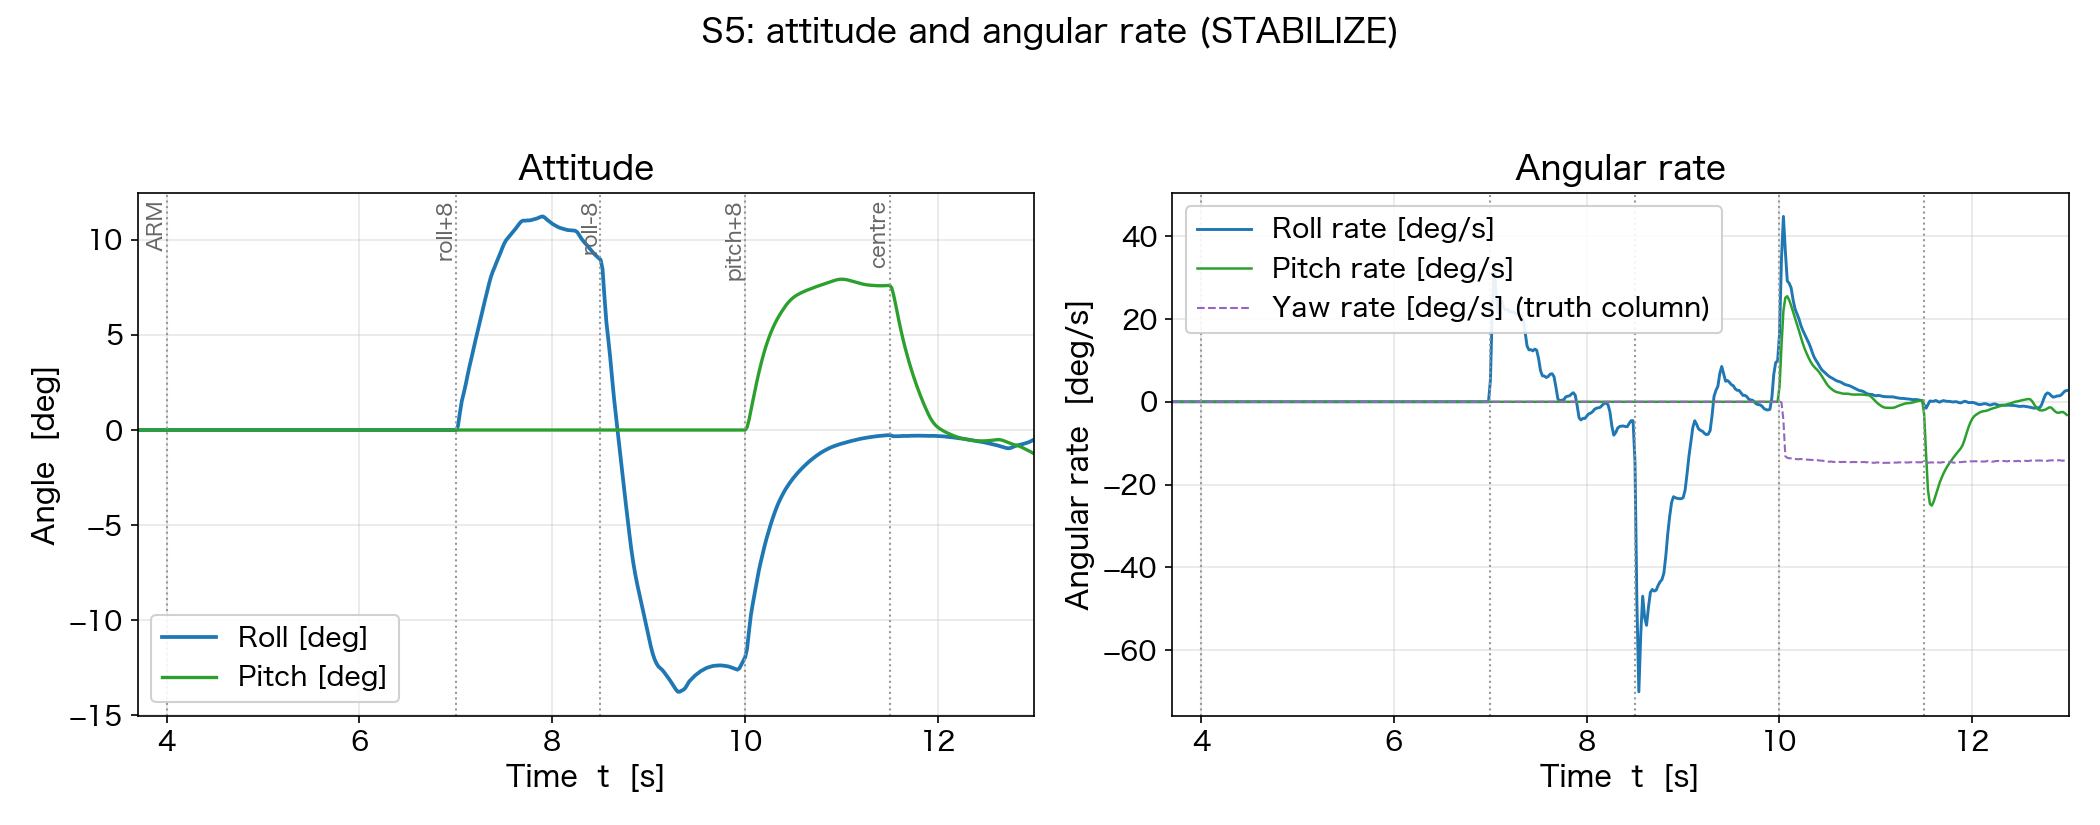
\includegraphics[width=\textwidth, height=0.68\textheight, keepaspectratio]{../fallback/S5_attitude_rate.png}
  \end{center}

  \vspace{0.3em}

  {\footnotesize \code{stab\_flight.scn}（vehicle）の姿勢角と角速度。12 項目の合否判定をすべて満たす}
\end{frame}

% ------------------------------------------------------------------
\begin{frame}[fragile]{解析ツール: sf log analyze / viz}
  \begin{block}{取得したテレメトリをそのまま解析する}\small
    \code{sf log wifi}/\code{sf log capture} で取得した CSV を，
    追加スクリプトなしで解析・可視化できる
  \end{block}

  \vspace{0.5em}

  \begin{sflisting}[basicstyle=\ttfamily\scriptsize]{コマンド}
sf log viz flight.csv
sf log analyze flight.csv
  \end{sflisting}

  {\footnotesize 詳しい手順は \code{docs/guides/flight-log-viz.md}。取得 $\to$ 可視化 $\to$
  解析の流れは S4 のシステム同定と同じログを使い回せる}
\end{frame}

% ------------------------------------------------------------------
\begin{frame}[fragile]{センサノイズの評価: Allan 分散\later}
  \begin{block}{Allan 分散でわかること}\small
    静止センサの出力から Allan 偏差（Allan deviation）を計算すると，
    ホワイトノイズと長時間のバイアス不安定性を分離して評価できる。
    ESKF の Q/R（プロセス／観測ノイズ共分散）チューニングの基礎データになる
  \end{block}

  \vspace{0.2em}

  \begin{sflisting}[basicstyle=\ttfamily\scriptsize]{コマンド}
sf log wifi -d 60 -o static_noise.csv   # 機体を静止させて60秒取得
sf sysid noise static_noise.csv --sensor gyro --static-only --plot
  \end{sflisting}

  \vspace{-1.5mm}

  {\footnotesize \code{--sensor} は \code{gyro/accel/baro/tof/all} を選べるが，
  \code{sf log wifi -o} の CSV は gyro/accel のみ。baro/tof には
  \code{sf log capture} $\to$ \code{sf log convert} を使う。
  トリム調整には \code{sf trim analyze} がある}
\end{frame}

% ------------------------------------------------------------------
% Author's 2nd-round review: the single "L1 Topic API" frame was too
% abrupt. Expanded into 3 \later frames so participants can read this at
% home: (a) what the Topic API is (real topic names from topics.hpp, real
% read functions from sf_api.hpp), (b) how to plug in your own estimator/
% controller (real IEstimator/IController methods, real swap mechanism),
% (c) a pointer to the example program. Accuracy note (checked against the
% headers directly): sf::api::* (sf_api.hpp, M2d scope) is READ-ONLY today
% — thin wrappers around Topic<T>::latest(). There is no publish-side
% entry point exposed to learners yet (actuator control / state requests
% are explicitly out of scope in the header's own comment). So frame (a)
% describes Topic<T> publish/latest as the underlying Pub-Sub mechanism
% used BETWEEN firmware components, and sf::api::* as the read-only subset
% exposed to L1. Frame (b) describes the actual swap path found in the
% task sources (imu_task.cpp's createEstimator() factory keyed on the
% estimator.type param; control_task.cpp's single static PidController
% instance for the controller side, since no controller factory exists
% yet).
% 著者の第2ラウンドレビュー: 「L1 Topic API」1枚は説明が急すぎた。3枚の
% \later フレームに拡張し，受講者が後で読めるようにした: (a) Topic API とは
% 何か（topics.hppの実トピック名，sf_api.hppの実読み取り関数），(b) 自分の
% 推定器・制御器を載せる方法（実際のIEstimator/IControllerメソッド，実際の
% 差替え機構），(c) サンプルプログラムへの導線。正確性の注記（ヘッダを直接
% 確認済み）: sf::api::*（sf_api.hpp, M2dスコープ）は現状「読み取り専用」—
% Topic<T>::latest() の薄いラッパーに過ぎない。学習者向けのpublish側の入口は
% まだ無い（アクチュエータ制御・状態要求はヘッダ自身のコメントで明示的に
% 対象外）。そこで(a)ではファームコンポーネント間で使われる本来のPub-Sub機構
% としてTopic<T>のpublish/latestを説明し，sf::api::*はL1に公開された読み取り
% 専用の部分集合と位置づける。(b)ではタスクソースで実際に見つかった差替え
% 経路を説明する（推定器はimu_task.cppのcreateEstimator()ファクトリが
% estimator.typeパラメータで分岐；制御器はcontrol_task.cppの単一static
% PidControllerインスタンスを直接差し替える — 制御器側にはまだファクトリが
% 無いため）。
\begin{frame}{研究利用の入口 (1/3): Topic API とは\later}
  \begin{block}{Pub-Sub（発行/購読型のメッセージ配信）}\footnotesize
    \code{Topic<T>}（\code{sf\_core}）がコンポーネント間を疎結合につなぐ。
    発行側は \code{publish(data)}，購読側は \code{latest()} で最新値を読む
  \end{block}

  \vspace{0.2em}

  \begin{table}
    \centering\scriptsize
    \begin{tabular}{ll}
      \hline
      \textbf{トピック（\code{sf::}名前空間）} & \textbf{内容} \\
      \hline
      \code{sensor\_imu}       & IMU 生データ（400\,Hz） \\
      \code{estimate\_state}   & 推定した姿勢・位置・速度 \\
      \code{command\_setpoint} & パイロット/API の目標値 \\
      \code{control\_output}   & 推力・トルク指令 \\
      \hline
    \end{tabular}
  \end{table}

  {\scriptsize 学習者向け読み取り関数（\code{sf::api::*}，\code{sf\_api.hpp}）:
  \code{imu\_latest()}/\code{estimate\_latest()}/\code{command\_latest()} など。
  \code{Topic<T>::latest()} をラップした\warn{読み取り専用}の入口（書き込み側は未公開）}
\end{frame}

% ------------------------------------------------------------------
\begin{frame}[fragile]{研究利用の入口 (2/3): 推定器・制御器を載せる\later}
  \begin{block}{\code{IEstimator}/\code{IController} を実装する}\footnotesize
    既存の ESKF・PID と同じインターフェース（\code{sf\_estimator}/\code{sf\_controller}）
    を実装すれば差し替えられる
  \end{block}

  \begin{table}
    \centering\scriptsize
    \begin{tabular}{ll}
      \hline
      \textbf{インターフェース} & \textbf{主なメソッド} \\
      \hline
      \code{IEstimator}  & \code{predict()}, \code{update*()}, \code{getState()}, \code{reset()} \\
      \code{IController} & \code{compute()}, \code{reset()}, \code{onModeChange()} \\
      \hline
    \end{tabular}
  \end{table}

  {\scriptsize \textbf{差替え手順:} 推定器は \code{estimator.type} パラメータで選ぶ
  （\code{imu\_task.cpp} の \code{createEstimator()} を拡張して自作を足す）。制御器は
  現状 PID の単一実装のみのため，\code{control\_task.cpp} の \code{static PidController
  controller;} を自分のクラスに置き換える（コントローラ側にはまだファクトリが無い）}
\end{frame}

% ------------------------------------------------------------------
\begin{frame}[fragile]{研究利用の入口 (3/3): サンプルプログラム\later}
  \begin{block}{\code{examples/09\_topic\_api\_hello}}\footnotesize
    姿勢トピックを購読し，roll/pitch/yaw を 10\,Hz でシリアル表示する最小例
  \end{block}

  \begin{sflisting}[basicstyle=\ttfamily\scriptsize]{抜粋（イメージ）}
sf::StateEstimate est = sf::api::estimate_latest();
auto rpy = sf::math::Quat(est.attitude[0], est.attitude[1],
                           est.attitude[2], est.attitude[3]).to_euler();
printf("roll=%.1f pitch=%.1f yaw=%.1f\n",
       rpy.x*180/M_PI, rpy.y*180/M_PI, rpy.z*180/M_PI);
  \end{sflisting}

  {\scriptsize ビルド: \code{idf.py set-target esp32s3 \&\& idf.py build} $\to$
  \code{idf.py -p <port> flash monitor}\\[2pt]
  \warn{帰宅後に再現:} \code{examples/09\_topic\_api\_hello}（\code{04\_read\_imu} 等と
  同じく単独ビルド可能）を手元で試す}
\end{frame}

% ------------------------------------------------------------------
\begin{frame}{再現性の3原則\later}
  \vspace{0.3em}

  {\small S1 で見た開発の3原則を，再現性の観点から振り返る}

  \vspace{0.3em}

  \begin{table}
    \centering\small
    \begin{tabular}{lp{80mm}}
      \hline
      \textbf{原則} & \textbf{内容} \\
      \hline
      Code Identity & SILS は実ファームと同じソースをそのままコンパイルして走る \\
      Parameter Identity & 同じパラメータで走らせる \\
      Model Fidelity & 実機飛行後にモデルをログで較正する（後追いの精度向上） \\
      \hline
    \end{tabular}
  \end{table}

  \vspace{0.5em}

  {\small パラメータは \code{param set}/\code{param save} で NVS に保存する。
  自作の推定器・制御器を試すときも，この3原則があるから「SILS で通った」が
  実機の挙動を意味する}
\end{frame}

% ------------------------------------------------------------------
\begin{frame}{発展テーマ: AI と強化学習\later}
  \begin{itemize}\small
    \item \textbf{AI コーディングエージェントの活用}: 制御則の実装・デバッグや
          シミュレーションログの解析を，AI コーディングエージェントを補助に
          進める流れが広がりつつある。StampFly のような小型・低リスクな
          実験プラットフォームは，その検証サイクルを高速に回す題材になりうる
    \item \textbf{強化学習と Sim-to-Real}: シミュレータ上で学習した制御方策を
          実機に転移する流れを教材化できれば，古典制御から学習型制御へ
          カリキュラムの射程が広がる。機体が小型・軽量で墜落時のリスクが
          小さいことは Sim-to-Real の実機検証に向く
  \end{itemize}
\end{frame}

% ------------------------------------------------------------------
\begin{frame}{発展テーマ: 制御・推定・自律飛行\later}
  \begin{itemize}\small
    \item \textbf{MPC・適応制御}: 今日扱った PID の先にある発展的な制御手法
    \item \textbf{ESKF・オートチューン}: 15状態 ESKF の実装，
          S4 で紹介した \code{sf\_autotune} によるオンボードチューニング
    \item \textbf{高度・位置ループ}: レート/姿勢カスケードの外側に
          ALT\_HOLD/POS\_HOLD が乗る。外乱オブザーバ（\code{altitude.dob.fc}）も
          パラメータで opt-in できる
    \item \textbf{Tello 互換 SDK と ROS 2}: Python SDK（\code{lib/stampfly}）と
          \code{sf takeoff} などの Tello 風コマンド（\code{sf takeoff/land/hover/jump} …）
          で自律飛行の入口を用意している。ROS 2 との連携も発展的なテーマの一つである
  \end{itemize}
\end{frame}

% ------------------------------------------------------------------
\begin{frame}{教育・研究での再利用\later}
  \begin{columns}[T]
    \begin{column}{0.5\textwidth}
      \begin{block}{自分の授業・研究室で使うには}\footnotesize
        \begin{itemize}
          \setlength{\itemsep}{1pt}
          \item \code{lesson\_manifest.yaml} の \code{courses:} に実習順序を
                追加できる（本チュートリアルの \code{sci2026} も同じ仕組み）
          \item 本スライド一式は LaTeX（Beamer）ソースごと公開されている
          \item SILS で実機なしの演習・採点も一部自動化できる
          \item Blockly・競技会（\code{sf blocks --demo}, \code{sf competition}）
                も用意している
        \end{itemize}
      \end{block}
    \end{column}
    \begin{column}{0.47\textwidth}
      \begin{exampleblock}{コミュニティへ}\footnotesize
        質問・不具合報告・開発への協力はリポジトリの Issue で受け付けている\\[4pt]
        \url{https://github.com/M5Fly-kanazawa/stampfly_ecosystem}
      \end{exampleblock}
    \end{column}
  \end{columns}
\end{frame}

% ------------------------------------------------------------------
\begin{frame}{理論とコードの対応表\later}
  {\footnotesize 本セッションの概念が，リポジトリのどのファイル・コマンドに対応するか一覧する}

  \vspace{0.3em}

  \resizebox{\textwidth}{!}{%
  \begin{tabular}{lll}
    \hline
    \textbf{概念} & \textbf{実装場所} & \textbf{コマンド} \\
    \hline
    層1: 設計用線形モデル       & \code{control/models/stampfly\_physical.yaml} & \code{sf sysid rate-fit} \\
    層2: 実ログ駆動オフライン再生 & \code{analysis/scripts/}                       & --- \\
    層3: SILS                   & \code{simulator/sils/}                         & \code{sf sils scenario} \\
    モデル一致の合否判定         & \code{tools/log\_analyzer/rate\_sysid.py}      & \code{sf sils sysid-gate} \\
    推定インターフェース         & \code{sf\_estimator} / \code{sf\_estimator\_eskf} & --- \\
    制御インターフェース         & \code{sf\_controller} / \code{sf\_controller\_pid} & --- \\
    \hline
  \end{tabular}}

  \vspace{0.5em}

  {\small 3層とも同じ物理パラメータ（\code{stampfly-parameters.md}）を参照する。
  層を追うごとにプラント物理・制御コードの忠実度が上がる}
\end{frame}

% ------------------------------------------------------------------
\begin{frame}{復習パス}
  \resizebox{\textwidth}{!}{%
  \begin{tabular}{lll}
    \hline
    \textbf{コマンド} & \textbf{扱う内容} & \textbf{文書} \\
    \hline
    \code{sf sim run vpython}  & VPython シミュレータ    & \code{simulator/README.md} \\
    \code{sf sils gui}         & SILS ブラウザ実験環境   & \code{simulator/sils/gui/README.md} \\
    \code{sf log viz}          & ログ可視化              & \code{docs/guides/flight-log-viz.md} \\
    ---                        & シミュレーション方針     & \code{docs/architecture/simulation-policy.md} \\
    \hline
  \end{tabular}}
\end{frame}

% ------------------------------------------------------------------
\begin{frame}{質疑}
  \begin{block}{想定質問}\small
    \begin{itemize}
      \item モデル一致の判定で Yaw 軸だけ精度が悪化するのはなぜか
      \item 自作の制御器を載せるとき，安全機構（フェイルセーフ）は
            どこまで自分で書く必要があるか
      \item ROS 2 と連携するにはどこから手を付ければよいか
    \end{itemize}
  \end{block}

  \vspace{0.5em}

  {\small 質疑の時間は本セッション末の15分。時間内に扱いきれなかった質問は，
  リポジトリの Issue で受け付けている}
\end{frame}

% ------------------------------------------------------------------
\begin{frame}{チェックポイント}
  \begin{alertblock}{確認事項}\small
    \begin{itemize}\setlength{\itemsep}{1pt}
      \item[$\square$] シミュレーションの3層構造と，それぞれの役割を説明できる
      \item[$\square$] \code{sf sils gui} でのシナリオ実行とパラメータ編集の流れを見た
            （または手元で試した）
      \item[$\square$] L1 Topic API で自分の推定器・制御器を差し替える方法を理解した
            （詳しくは「研究利用の入口 (1/3)〜(3/3)」）
      \item[$\square$] 解析ツールの入口を把握した
    \end{itemize}
  \end{alertblock}

  \vspace{0.2em}

  \begin{block}{本日はこれで終了}
    資料・録画は公開されている。持ち帰り資料（付録）で復習を続けられる
  \end{block}
\end{frame}
